\subsection{Arduino based DAQ}
\subsubsection{Arduino Code}
Introduce Code
% Arduino code flowchart
\begin{figure}[htbp] %h-ere t-op b-ottom p-page (separte) -good to allow all htbp to give the compiler more options
  \centering
  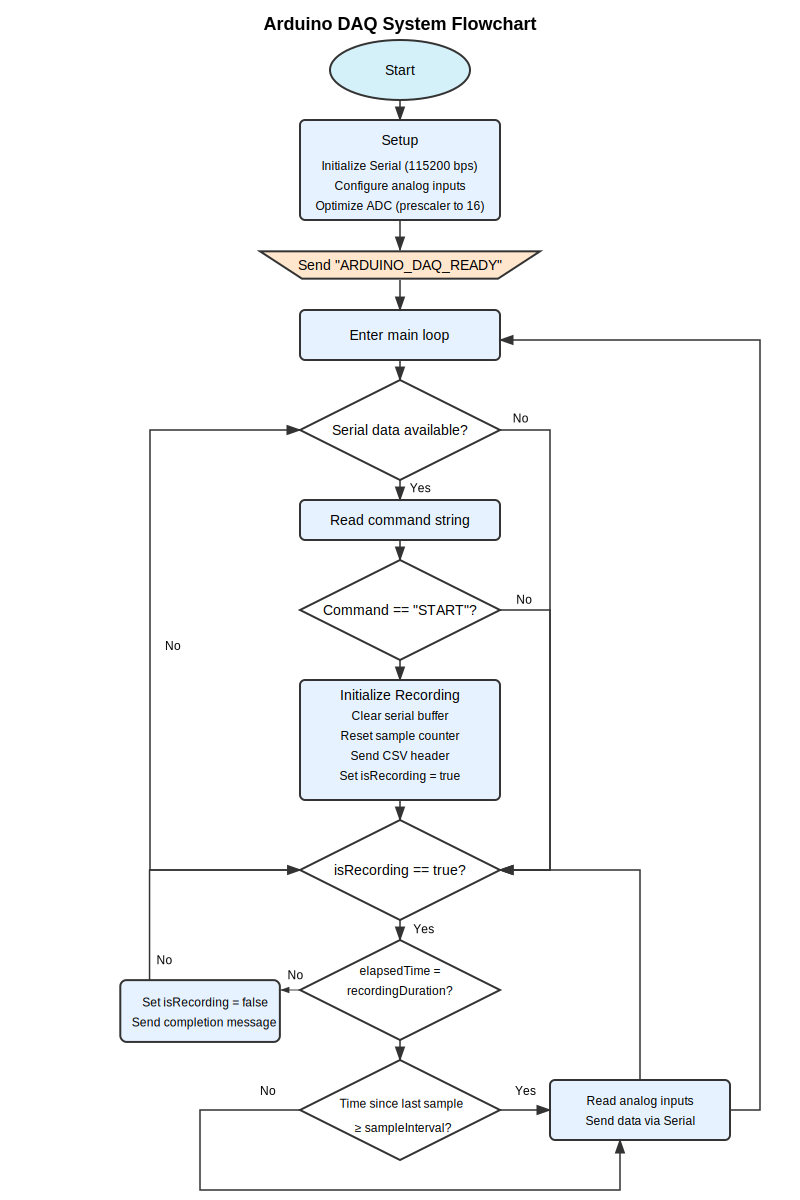
\includegraphics[width=0.6\textwidth]{chapters/methodology/ArduinoDAQ/flowchart_Arduino_code.png} % change {path}
  \caption{Flowchart of C++ code on Arduino DAQ}      
  \label{fig:daq_arduino_code}           
\end{figure}                            
\paragraph{Sampling Rate}
Several factors restrict the sampling rate:

\subparagraph{Sample Interval Setting}
The most direct limitation is the \texttt{sampleInterval} constant set to 2ms in the code, which means samples are taken no more frequently than every 2 milliseconds (500 Hz theoretical maximum).

\subparagraph{ADC Prescaler Configuration}
The ADC prescaler is set to 16 (from the default of 128) with this line:
\begin{verbatim}
ADCSRA = (ADCSRA & 0xF8) | 0x04;
\end{verbatim}
This increases the ADC clock to 16MHz/16 = 1MHz. With each conversion taking 13 ADC clock cycles, the theoretical maximum sampling rate is about 76.9kHz for a single channel.

\subparagraph{Multiple Channel Reading}
Since the system reads from 4 analog inputs sequentially, the effective per-channel sampling rate is reduced by approximately a factor of 4.

\subparagraph{Serial Transmission Overhead}
Each sample requires formatting and sending data over serial:
\begin{verbatim}
String dataString = String(sampleCount) + "," + String(elapsedTime);
// ... format and add voltage values ...
Serial.println(dataString);
\end{verbatim}
This string creation and serial transmission takes considerable time.

\subparagraph{Serial Baud Rate}
The code uses 115200 bps, which limits how quickly data can be transmitted. Each sample in this format might be around 30-40 bytes, which means \texttildelow 3000-3800 samples/second theoretical maximum throughput.

\subparagraph{String Operations}
The use of the Arduino \texttt{String} class is memory-intensive and can cause fragmentation over time, potentially causing slowdowns.

\subparagraph{Loop Cycle Time}
Other operations in the main loop consume processing time.

The dominant limiting factor in this implementation is likely the combination of the explicit 2ms sample interval and the serial communication overhead. Higher sampling rates would require optimizing the data transmission format, possibly using binary rather than text formatting, and reducing the sample interval.